\section{Subsistema: Alimentação} \label{sec:alimentacao}

\par O subsistema de alimentação do carrinho de compras autônomo compreende além dos  motores, que serão acoplados nas rodas traseiras, baterias para garantir alimentação para a movimentação do carrinho e o funcionamento dos componentes eletrônicos e um carregador para a bateria.
\par Os motores de corrente contínua de 12 V serão alimentados por uma bateria com a mesma tensão, garantindo uma autonomia da até duas horas para que o usuário possa carregar as  compras do supermercado.
\par Para que seja possível fazer um comparativo de forma quantitativa dos tipos de motores e baterias mais viáveis de serem utilizados, adotou-se alguns critérios e seus respectivos pesos, de acordo com a importância para o projeto, que são listados na Tabela \ref{tab:indicadores-escolha}.
\par Para fazer esse comparativo utilizou-se indicadores que determinam os critérios mais importantes na escolha dos componentes.Nesse caso o indicador com maior valor é o custo,pois o projeto conta com um baixo orçamento,utilizou-se outros indicadores para garantir a qualidade do produto mesmo este contar com um baixo orçamento.
\par Os outros indicadores utilizados para o comparativo foram eficiência,integração com os subsistemas do produto,tamanho,massa e manutenção.Para esta comparação foram atribuídos pesos de acordo com a importância de cada indicador para o projeto,estes pesos foram determinados pelos autores.Para esses indicadores atribuiu-se um peso normalizado para cada,este valor foi determinado do seguinte modo 

\begin{table}[h]
\centering
\caption{Indicadores para formalizar um critério de escolha.}
\label{tab:indicadores-escolha}
\begin{tabular}{ccc}
\rowcolor[HTML]{000000} 
{\color[HTML]{FFFFFF} Critérios do Projeto}               & {\color[HTML]{FFFFFF} Pesos} & {\color[HTML]{FFFFFF} Pesos Normalizados} \\
\cellcolor[HTML]{000000}{\color[HTML]{FFFFFF} Custo}      & 10                           & 0,3225                                   \\
\cellcolor[HTML]{000000}{\color[HTML]{FFFFFF} Integração} & 7                            & 0,2258/                                   \\
\cellcolor[HTML]{000000}{\color[HTML]{FFFFFF} Tamanho}    & 6                            & 0,1935                                   \\
\cellcolor[HTML]{000000}{\color[HTML]{FFFFFF} Massa}      & 4                            & 0,1290                                   \\
\cellcolor[HTML]{000000}{\color[HTML]{FFFFFF} Manutenção} & 4                            & 0,1290                                  \\
{\color[HTML]{000000} \textbf{Total}}                     & 38                           & 1                                        
\end{tabular}
\end{table}

\subsection{Motores}

%os tópicos a seguir esclarecem sobre os estudos realizados a fim de se tomar decisões sobre motores.
\par O motor está entre os componentes de maior importância para este projeto, já que ele será o responsável pelo deslocamento do carrinho de compras. Assim, fez-se uma pesquisa	de comparação entre os motores já utilizados em grande escala no mercado.
Para o projeto do carrinho de compras, optou-se por usar um sistema propulsor elétrico, pois este combina as vantagens da utilização de energia elétrica	, baixo custo, facilidade de transporte e simplicidade no comando. \cite{maqel}
\par Sabe-se que os motores elétricos são divididos entre motor de corrente contínua (CC) e motor de corrente alternada (CA). Escolheu-se o motor de corrente contínua devido a algumas vantagens em relação ao outro, como ampla faixa de variação de velocidade, simplicidade de manutenção e baixo custo. Além disso, não é necessário possuir equipamentos intermediários para que se alterne o sinal de saída contínuo das baterias, como inversores.
\par Com isso, dentre os aspectos analisados para a escolha do modelo do motor a ser utilizado, estão:
\par•	Elevado torque de partida a velocidades baixas;
\par•	Facilidade no controle de velocidade;
\par•	Eficiência.
\par•	Funcionamento contínuo, inclusive a baixas rotações;
\par•	Características físicas, como tamanho e peso;

\par A Figura \ref{fig:curvas_motor} mostra as curvas características dos motores CC. Nela, é possível observar que a corrente será praticamente constante, variando apenas durante as acelerações provocadas pelo aumento da tensão, em que a corrente, transitoriamente, aumenta para provocar a aceleração da máquina. Portanto, em regime, o motor CC opera a corrente de armadura essencialmente constante também. Assim, o motor tem disponibilidade de acionar a carga exercendo um torque constante, podendo ser em qualquer rotação, desde que seja até o limite nominal, o que indica uma corrente de armadura nominal \cite{prentice}.

\begin{figure}[ht]
		\centering
		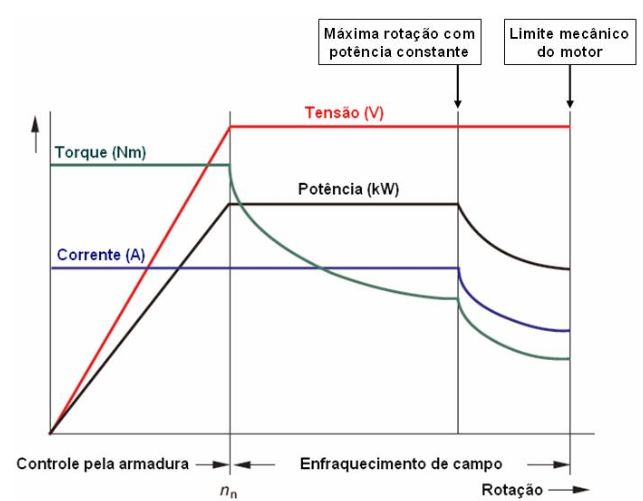
\includegraphics[width=0.6\textwidth]{figuras/curvamotorcc.JPG}
		\caption{Curvas características de um motor CC.  Fonte: \citeauthor{prentice} (\citeyear{prentice}).}
		\label{fig:curvas_motor}
\end{figure} 


\subsection{Dimensionamento do motor}
\par Antes de fazer a escolha do motor elétrico, foram feitos cálculos para saber a potência necessária para as condições iniciais, bem como cálculos do torque e da velocidade de rotação. 
\par Assim, determinou-se que o carrinho de compras irá andar com velocidade máxima de 5 km/h (1,38889m/s) com um tempo de aceleração de 3s. A partir disso, é possível obter a aceleração do sistema, considerando que o carrinho esteja parado e atinja uma velocidade final em um determinado intervalo de tempo, de acordo com a equação abaixo.

$$ a=  \frac{(V_f-V_o)}{t}   $$ 

\par Então,

$$ a =  1,38889/3 = 0,462963 \quad m/s^2 $$ 

\par Estipulou-se que a massa total do sistema (carrinho + compras) será de no máximo 50Kg. Dessa forma, foi possível determinar a força necessária para acelerar o carrinho, expressa em Newtons (N), mostrada na equação abaixo.

$$ F_a = m*a = 50*0,462963 = 23,14815 \quad N $$

\par Para encontrar a força total do sistema, é necessário saber a força de resistência ao arraste, que corresponde ao valor contrário à força do motor. A força de resistência ao arraste é dada pela equação abaixo, em que g é a aceleração da gravidade e $\mu_c$ corresponde ao coeficiente de atrito estático do pneu com asfalto, tabelado.

$$ F_r = \mu_c*m*g = 0,3*50*9,81   $$
$$ F_r = 147,15 \quad N $$
		A força total é dada pela equação abaixo.
$$ F_t = F_a + F_r $$
Então,$$ F_t = 170,2981 \quad N   $$
		Assim, pode-se encontrar o torque necessário para movimentar o carrinho. A equação a seguir mostra a relação que possibilita esse cálculo.
$$ T = F_t*r $$
Onde r é o raio da roda do carrinho dado em metros. Assim, o torque será:
$$ T = 170,2981*0,06 = 10,22 \quad N.m $$
		A potência necessária para auxiliar a movimentação do carrinho, expressa em Watts (W), é dada pela equação abaixo.
$$ P = F_t*V_f = 170,2981*1,38889 = 236,5 \quad W $$
		Por fim, calculou-se a velocidade de rotação do motor, expressa em rotações por minuto (rpm), como mostra a equação a seguir.
$$ Ns = \frac{V_f}{r}*\frac{60}{2\pi} $$
$$ Ns = (\frac{1.38889}{0.06})*(\frac{60}{2\pi}) = 221 \quad rpm $$


\subsection {Bateria}
\par Para o funcionamento do carrinho de compras autônomo, fez-se necessário o uso de uma bateria, capaz de suprir a necessidade de 250 W. Partindo dessa premissa, buscou-se baterias que pudessem atender os requisitos do projeto.


\subsubsection {Tipos de bateria}
\par As baterias mais comumente utilizadas e encontradas no mercado são as baterias de níquel cádmio, metal hidreto, chumbo ácido e lítio-íon, sendo utilizadas nas mais diversas aplicações, desde aparelhos eletrônicos portáteis, até veículos elétricos.\cite{Costa}

\begin{itemize} 

\item\textbf {Bateria de Níquel Cádmio}

\par Essas baterias são amplamente utilizadas em equipamentos portáteis, como câmeras de vídeo, telefones móveis e equipamentos médicos.O período de carga é curto, se comparado a outros tipos de bateria e a descarga é lenta. Esse tipo de bateria também apresenta número elevado de ciclos de carga e descarga e têm um baixo custo. Como desvantagens pode-se citar que este tipo de bateria é muito poluente e apresenta o efeito memória, fazendo com que as baterias não carreguem até o fim e apresentem ciclo de vida reduzido.


\item\textbf {Bateria de Chumbo ácida} 
\par São baterias econômicas, utilizadas em automóveis, no-breaks, equipamentos hospitalares e cadeiras de rodas elétricas. Estas foram as primeiras baterias de uso comercial.Entre as vantagens, apresenta 
custo baixo, não apresentam efeito memória e podem trabalhar em condições de grandes variações de temperatura. Apesar destas vantagens, são baterias pesadas e demoram para carregar, apresentam limitado número de ciclos e têm densidade de energia baixa, se comparada a outros tipos de bateria, também são poluentes.
 

\item \textbf{ Bateria de Níquel Metal Hidreto}
\par Esse tipo de bateria apresenta alta densidade de energia, em comparação com baterias de níquel cádmio, porém com ciclo de vida menor. São utilizadas em notebooks, telefones celulares e câmeras digitais.As maiores vantagens são apresentar capacidade maior que as baterias de níquel cádmio, o efeito memória é menor e não é tóxica. Entre as desvantagens estão a descarga profunda e repetidos ciclos reduzem a vida útil, apresenta corrente de descarga limitada e o processo de carga é mais complexo. Se comparado com as baterias de níquel cádmio estas se auto descarregam mais rapidamente, são mais caras e necessitam de mais manutenção. 


\item\textbf{Bateria de Lítio íon}
É uma bateria leve, e fornece alta densidade de energia por peso. É a bateria que mais está crescendo. Uma das vantagens é a densidade de energia elevada e auto descarga e a manutenção são baixas. As desvantagens são que a corrente de descarga é moderada, o custo é um pouco elevado, a tecnologia ainda não está totalmente madura. 
\end{itemize}


\subsection{Dimensionamento da bateria}

\par Considerando que o carrinho será movimentado através de dois motores de 250 W, acoplados às rodas traseiras do carrinho autônomo e já considerando uma faixa de segurança para a alimentação dos componentes eletrônicos, dimensionou-se a bateria, de 12 V, por ser a mesma tensão da maioria de opções de motores, não havendo a necessidade de transformar a tensão para alimentar os motores, simplificando assim o projeto.
\par Considerando que os motores não irão necessitar da potência total, ou seja, a potência máxima requeria é de 250 W. Para a alimentação dos componentes eletrônicos, estima-se que a potência requerida é de 5 W. Utilizando os valores de potência e tensão pré determinados, calculou-se a corrente necessária:

$$ P= U*I$$
$$ I={P}*{U} $$
$$ I=\frac{255}{12}$$
$$ I= 21,25 A$$

\par Deste modo, a corrente exigida pelos motores, já considerando os componentes eletrônicos é de 21,25 A.
\par Considerando autonomia de 2 horas do carrinho autônomo, calcula-se a capacidade da bateria:

$$ Capacidade = 21.25*2$$
$$ Capacidade = 42.5 Ah $$

\par Assim, a capacidade da bateria é de 42.5 Ah, porém não é recomendada a descarga total, uma vez que isto diminui a vida útil da bateria. Considerando uma profundidade de descarga de 70 por cento, calculou-se a capacidade para a bateria:

$$ Ah={42.5}/{0.7}$$
$$ Ah= 60.71 $$


\par Esta capacidade da bateria considera os motores operando na potência máxima, ou seja, considerando a potência necessária para manter o carrinho em movimento, partindo da inércia, durante as duas horas definidas como requisito.  Porém, o carrinho não opera nesta potência em todo o tempo de funcionamento devido a alguns fatores. Entre eles estão o fato de que este não opera sempre com a máxima capacidade de massa, em alguns momentos ele fica parado e quando está em movimento necessita de força apenas para vencer a força de atrito dinâmica e não mais a inércia do sistema.
\par Assim, considerando a capacidade total calculada anteriormente de 60,71 Ah, para um fator de demanda do motor estimado de 0,65:

$$ Ah= 60.71*0.65$$
$$ Ah=39.46 $$


\par Sendo assim, a bateria necessária para o funcionamento do carrinho de compras autônomo deve ter a capacidade de 40 Ah. 
\par Para a escolha da bateria a ser utilizada levou-se em conta principalmente o custo e a facilidade para aquisição. Levando tudo isso em conta e analisando as vantagens e desvantagens de cada tipo, optou-se pela bateria selada de chumbo ácido, por ter muitas opções no mercado, refletindo em maior facilidade de compra, ser uma tecnologia madura, apresentar menor custo e amplo uso em diversos produtos, como cadeiras de rodas automáticas e veículos Elétricos de pequeno porte.

\subsection{Carregador da bateria}

\par Os carregadores de bateria podem ser de dois tipos, de carga cíclica ou de flutução. O primeiro tipo é utilizado para carregar baterias automotivas descarregadas ou para carregar totalmente uma bateria para alimentar um equipamento isolado. Durante a carga da bateria, esta não deve alimentar nenhum aparelho, pois a tensão pode aumentar para até 14,8 V, podendo assim, danificar o equipamento.
\par O carregador de flutuação permite que a bateria alimente equipamentos enquanto carrega, uma vez que opera com tensão de carga mais baixa, de até 13,8V, que é chamada tensão de flutuação. 

\subsubsection{Métodos de carga da bateria}
\par Para baterias de chumbo-ácido, há três diferentes métodos de carga, que consistem em aplicar corrente constante, tensão constante ou potência constante. Com esses parâmetros é possível utilizar métodos variados de carregamento, sendo possível determinar qual dos três parâmetros será controlado.
\par Os métodos mais utilizados, encontrados na literatura são listados a seguir:

\begin{itemize}
\item Método a um nível de corrente e um nível de tensão: 
\par Este método é o mais utilizado devido à facilidade de implementação. Consiste em dois estados, onde o primeiro a corrente se mantem constante até que a tensão da bateria atinja a tensão de flutuação e no segundo estado aplica-se a tensão de flutuação na bateria para que esta possa manter sua carga.
\item Método duplo nível de tensão:
\par Este método consiste em três etapas. Na primeira etapa é aplicada uma corrente constante até que a tensão sobre a bateria alcance a tensão de equalização.Na segunda etapa a tensão de equalização se mantem constante sobre a bateria, no final desta etapa a bateria obtêm 100 por cento de carga. Já no terceiro estágio, se aplica a tensão de flutuação, mantendo-se constante sobre a bateria, para que esta conserve sua carga.
\item Métodos duplo nível de corrente:
\par Este método consiste em dois estágios de aplicação de corrente,  onde o nível desta corrente é controlado a partir do nível de tensão. No primeiro estágio, aplica-se uma corrente até que a tensão da bateria alcance a tensão de equalização, já o segundo estágio tem como função manter a carga da bateria, onde aplica-se uma corrente pulsante de retenção, para manter a tensão de flutuação constante.
\item Método de corrente pulsada: 
\par Este método consiste em dois estágios de aplicação de corrente. No primeiro estágio, aplica-se um corrente constante até que a tensão atinja a tensão de equaliação. O segundo estágio consiste em monitorar a tensão da bateria, ou seja, quando a tensão de flutuação diminui, aplica-se novamente uma corrente para que a tensão volte a tensão de equalização, isto se repete caracterizando-se uma corrente pulsante sobre a bateria, mantendo-se assim a sua carga. 

\end{itemize}

\subsubsection{Componentes do carregador}
 \par Para a fabricação de um carregador de baterias é necessário alguns componentes, destacando-se o transformador e a ponte retificadora.
\begin{itemize}
\item Transformador: Diminui o nível de tensão da rede elétrica para o nível de tensão da bateria.
\item Ponte retificadora: Transforma a tensão alternada para tensão contínua. 

\end{itemize}
\par A Figura \ref{fig:diagrama_carregador} apresenta um esquema dos componentes de um carregador de baterias.  
\begin{figure}[ht]
		\centering
		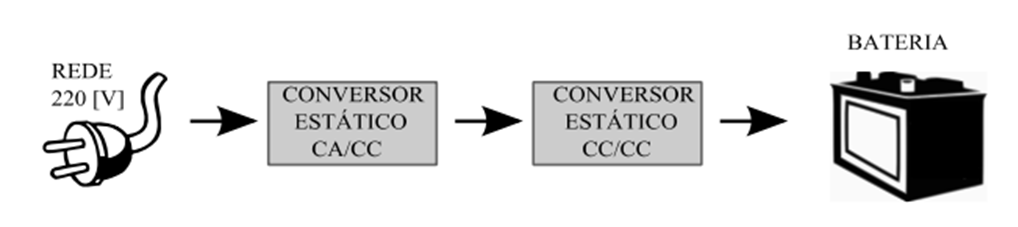
\includegraphics[width=1\textwidth]{figuras/imagem.png}
		\caption{Diagrama de blocos dos componentes do carregador de baterias}
		\label{fig:diagrama_carregador}
\end{figure} 






							
